\documentclass[10pt]{beamer}\usepackage[]{graphicx}\usepackage[]{color}
% maxwidth is the original width if it is less than linewidth
% otherwise use linewidth (to make sure the graphics do not exceed the margin)
\makeatletter
\def\maxwidth{ %
  \ifdim\Gin@nat@width>\linewidth
    \linewidth
  \else
    \Gin@nat@width
  \fi
}
\makeatother

\definecolor{fgcolor}{rgb}{0.345, 0.345, 0.345}
\newcommand{\hlnum}[1]{\textcolor[rgb]{0.686,0.059,0.569}{#1}}%
\newcommand{\hlstr}[1]{\textcolor[rgb]{0.192,0.494,0.8}{#1}}%
\newcommand{\hlcom}[1]{\textcolor[rgb]{0.678,0.584,0.686}{\textit{#1}}}%
\newcommand{\hlopt}[1]{\textcolor[rgb]{0,0,0}{#1}}%
\newcommand{\hlstd}[1]{\textcolor[rgb]{0.345,0.345,0.345}{#1}}%
\newcommand{\hlkwa}[1]{\textcolor[rgb]{0.161,0.373,0.58}{\textbf{#1}}}%
\newcommand{\hlkwb}[1]{\textcolor[rgb]{0.69,0.353,0.396}{#1}}%
\newcommand{\hlkwc}[1]{\textcolor[rgb]{0.333,0.667,0.333}{#1}}%
\newcommand{\hlkwd}[1]{\textcolor[rgb]{0.737,0.353,0.396}{\textbf{#1}}}%
\let\hlipl\hlkwb

\usepackage{framed}
\makeatletter
\newenvironment{kframe}{%
 \def\at@end@of@kframe{}%
 \ifinner\ifhmode%
  \def\at@end@of@kframe{\end{minipage}}%
  \begin{minipage}{\columnwidth}%
 \fi\fi%
 \def\FrameCommand##1{\hskip\@totalleftmargin \hskip-\fboxsep
 \colorbox{shadecolor}{##1}\hskip-\fboxsep
     % There is no \\@totalrightmargin, so:
     \hskip-\linewidth \hskip-\@totalleftmargin \hskip\columnwidth}%
 \MakeFramed {\advance\hsize-\width
   \@totalleftmargin\z@ \linewidth\hsize
   \@setminipage}}%
 {\par\unskip\endMakeFramed%
 \at@end@of@kframe}
\makeatother

\definecolor{shadecolor}{rgb}{.97, .97, .97}
\definecolor{messagecolor}{rgb}{0, 0, 0}
\definecolor{warningcolor}{rgb}{1, 0, 1}
\definecolor{errorcolor}{rgb}{1, 0, 0}
\newenvironment{knitrout}{}{} % an empty environment to be redefined in TeX

\usepackage{alltt}


%\input{slides_header.tex}
\usepackage{graphicx}
\usepackage{hyperref, url}
\hypersetup{colorlinks,citecolor=myorange,filecolor=red,linkcolor=brown,urlcolor=blue}

\usepackage{longtable,booktabs}
\usepackage{amssymb,amsmath}
\usepackage{animate}
\usepackage{subfig}
\usepackage{tikz}
\usetikzlibrary{shapes.geometric, arrows,shapes.symbols,decorations.pathreplacing}
\tikzstyle{startstop} = [rectangle, rounded corners, minimum width=3cm, minimum height=1cm, draw=black, fill=pinkish,text width=3.5cm]
\tikzstyle{startstop2} = [rectangle, rounded corners, minimum width=3cm, minimum height=1cm, draw=black, fill=background,text width=4.5cm]
\tikzstyle{startstop3} = [rectangle, rounded corners, minimum width=3cm, minimum height=1cm, draw=black, fill=beige,text width=3.0cm]
\tikzstyle{startstop4} = [rectangle, rounded corners, minimum width=3cm, minimum height=1cm, draw=black, fill=pinkish,text width=4.5cm]
\tikzstyle{io} = [trapezium, trapezium left angle=70, trapezium right angle=110, minimum width=2cm, minimum height=1cm, text centered, draw=black, fill=blue!30,text width=1.5cm]
\tikzstyle{process} = [rectangle, minimum width=1cm, minimum height=1cm, text centered, draw=black, fill=orange!30,text width=2cm]
\tikzstyle{decision} = [diamond, minimum width=2cm, minimum height=1cm, text centered, draw=black, fill=green!30]
\tikzstyle{arrow} = [thick,->,>=stealth]
\tikzstyle{both} = [thick,<->,>=stealth, red]


% used for tree of stats tests in 001-introduction
\tikzstyle{startstopstats} = [rectangle, rounded corners, minimum width=2cm, minimum height=.5cm,text centered, draw=black, fill=red!30]
\tikzstyle{iostats} = [trapezium, trapezium left angle=70, trapezium right angle=110, minimum width=2cm, minimum height=.5cm, text centered, draw=black, fill=blue!30]
\tikzstyle{processstats} = [rectangle, minimum width=1.5cm, minimum height=.5cm, text centered, draw=black, fill=orange!30]
\tikzstyle{processbigstats} = [rectangle, minimum width=1.5cm, minimum height=.5cm, text centered, draw=black, fill=orange!30,text width=1.6cm]
\tikzstyle{decisionstats} = [rectangle, minimum width=1cm, minimum height=1cm, text centered, draw=black, fill=green!30,text width=1.6cm]
\tikzstyle{decisionbigstats} = [rectangle, minimum width=1cm, minimum height=1cm, text centered, draw=black, fill=yellow!30,text width=2cm]

\usepackage{pifont}% http://ctan.org/pkg/pifont
\newcommand{\cmark}{\ding{51}}%
\newcommand{\xmark}{\ding{55}}%

\usepackage{ulem} % for strikeout

\usepackage{xcolor}
\usepackage{color, colortbl}
\definecolor{lightgray}{RGB}{200,200,200}
\definecolor{palegray}{RGB}{221,221,221}
\definecolor{myblue}{RGB}{0,89,179}
\definecolor{myorange}{rgb}{0.776,0.357,0.157}
\definecolor{gray}{RGB}{110,110,110}
\definecolor{darkgray}{RGB}{100,100,100}
\definecolor{lightgray}{RGB}{200,200,200}
\definecolor{palegray}{RGB}{221,221,221}
\definecolor{turquoise}{RGB}{81,193,188}
\definecolor{tomato}{RGB}{255,136,136}
\definecolor{mandarina}{RGB}{229,169,25}
\definecolor{foreground}{RGB}{81,141,193}
\definecolor{background}{RGB}{246,244,240}
\definecolor{highlight}{RGB}{229,169,25}
\definecolor{lowlight}{RGB}{200,200,200}
\definecolor{beige}{RGB}{255,255,240}
\definecolor{pinkish}{RGB}{255,223,247}
\definecolor{darktangerine}{rgb}{1.0, 0.66, 0.07}
\definecolor{deepink}{RGB}{255,20,147}
%\usepackage{shadethm}
%\colorlet{shadecolor}{blue!15}
%\colorlet{shadecolor}{palegray}
%\setlength{\shadeboxrule}{.4pt}

%\newshadetheorem{thm}{Theorem}
%\newshadetheorem{defm}{Definition}
%\newshadetheorem{exm}{Exercise}
%\newshadetheorem{remarkm}{Remark}
%\definecolor{shadethmcolor}{HTML}{EDF8FF}
%\definecolor{shadethmcolor}{RGB}{221,221,221}
%\definecolor{shaderulecolor}{HTML}{45CFFF}
%\definecolor{shaderulecolor}{RGB}{0,89,179}
%\setlength{\shadeboxrule}{.4pt}



\usepackage{epsfig}

\newcommand{\code}[1]{\texttt{#1}}
\newcommand{\blue}[1]{\textcolor{blue}{#1}}
\newcommand{\red}[1]{\textcolor{red}{#1}}

\usepackage{comment}

\makeatletter

\def \iqsssectiontitleheader {}

\newcommand{\iqsssectiontitle}[1]{
	\def \iqsssectiontitleheader{#1}
}

\@ifundefined{insertmainframenumber}
{%
	% \insertmainframenumber not defined
	\newcommand{\insertmainframenumber}{\inserttotalframenumber}
}
{%
	% \insertmainframenumber already defined
}%


\AtBeginSection[]{
	\title{\insertsectionhead}
	{
		%\definecolor{white}{RGB}{140,193,250}
		%\definecolor{white}{RGB}{200,200,200}
		%\definecolor{white}{RGB}{242,244,247}
		\definecolor{white}{RGB}{0,89,179}
		%\definecolor{iqss@orange}{rgb}{1,1,1}
		\ifnum \insertmainframenumber > \insertframenumber
		%\setbeamercolor{background canvas}{bg=myblue}
		%\setbeamercolor{normal text}{fg=black,bg=white}
		%\setbeamercolor{frametitle}{fg=red}
		%\setbeamercolor{section in toc}{fg=myblue, bg=white}
		%\setbeamercolor{subsection in toc}{fg=myblue, bg=white}
		\frame{
			\frametitle{\iqsssectiontitleheader}
			\tableofcontents[currentsection]
		}
		\else
		\frame{
			\frametitle{Backup Slides}
			\tableofcontents[sectionstyle=shaded/shaded,subsectionstyle=shaded/shaded/shaded]
		}
		\fi
	}
}
\makeatother
%\graphicspath{{/home/sahir/git_repositories/EPIB607/resources/assets/slides/figure/}}


\usepackage{fontspec}
%\setsansfont{Fira Sans}
%\setmonofont{Fira Mono}
%\setsansfont[ItalicFont={Fira Sans Light Italic},BoldFont={Fira Sans},BoldItalicFont={Fira Sans Italic}]{Fira Sans Light}
%\setmonofont[BoldFont={Fira Mono Medium}]{Fira Mono}

\def\installpath{/usr/local/share/texmf/fonts/opentype/libertinus/}
\setmainfont{LibertinusSerif}[
UprightFont    = *-Regular,
BoldFont       = *-Bold,
ItalicFont     = *-Italic,
BoldItalicFont = *-BoldItalic,
Ligatures      = TeX,
Extension      = .otf,
Path           = \installpath/
]

\setsansfont{LibertinusSerif}[
UprightFont    = *-Regular,
BoldFont       = *-Bold,
ItalicFont     = *-Italic,
BoldItalicFont = *-BoldItalic,
Ligatures      = TeX,
Extension      = .otf,
Path           = \installpath/
]


%\setmonofont{LibertinusSerif}[
%UprightFont    = *-Regular,
%BoldFont       = *-Bold,
%ItalicFont     = *-Italic,
%BoldItalicFont = *-BoldItalic,
%Ligatures      = TeX,
%Extension      = .otf,
%Path           = \installpath/
%]






\newcommand\Wider[2][3em]{%
	\makebox[\linewidth][c]{%
		\begin{minipage}{\dimexpr\textwidth+#1\relax}
			\raggedright#2
		\end{minipage}%
	}%
}


\newcommand {\framedgraphic}[1] {
	\begin{figure}
		\centering
		\includegraphics[width=\textwidth,height=0.9\textheight,keepaspectratio]{#1}
	\end{figure}
}


\newcommand {\framedgraphiccaption}[2] {
	\begin{figure}
		\centering
		\includegraphics[width=\textwidth,height=0.8\textheight,keepaspectratio]{#1}
		\caption{#2}
	\end{figure}
}




\setbeamercolor{itemize item}{fg=myblue}
\setbeamercolor{itemize subitem}{fg=myorange}
%\setbeamertemplate{itemize item}[square]
\setbeamertemplate{itemize item}[circle]
\setbeamertemplate{itemize subitem}[triangle]
\setbeamertemplate{blocks}[rounded][shadow=true]
\setbeamercolor{block body alerted}{bg=alerted text.fg!10}
\setbeamercolor{block title alerted}{bg=alerted text.fg!20}
\setbeamercolor{block body}{bg=structure!10}
\setbeamercolor{block title}{bg=structure!20}
\setbeamercolor{block body example}{bg=green!10}
\setbeamercolor{block title example}{bg=green!20}


\makeatletter
\newenvironment<>{proofs}[1][\proofname]{%
	\par
	\def\insertproofname{#1\@addpunct{.}}%
	\usebeamertemplate{proof begin}#2}
{\usebeamertemplate{proof end}}
\newenvironment<>{proofc}{%
	\setbeamertemplate{proof begin}{\begin{block}{}}
		\par
		\usebeamertemplate{proof begin}}
	{\usebeamertemplate{proof end}}
	\newenvironment<>{proofe}{%
		\par
		\pushQED{\qed}
		\setbeamertemplate{proof begin}{\begin{block}{}}
			\usebeamertemplate{proof begin}}
		{\popQED\usebeamertemplate{proof end}}
\makeatother


\makeatletter
\newenvironment<>{exams}[1][\proofname]{%
	\par
	\def\insertproofname{#1\@addpunct{.}}%
	\usebeamertemplate{example begin}#2}
{\usebeamertemplate{example end}}
\newenvironment<>{examc}{%
	\setbeamertemplate{exam begin}{\begin{block}{}}
		\par
		\usebeamertemplate{exam begin}}
	{\usebeamertemplate{exam end}}
	\newenvironment<>{exame}{%
		\par
		\pushQED{\qed}
		\setbeamertemplate{exam begin}{\begin{block}{}}
			\usebeamertemplate{exam begin}}
		{\popQED\usebeamertemplate{exam end}}
		\makeatother

%\definecolor{mycolor}{HTML}{F7F8E0}
%\declaretheorem[shaded={bgcolor=mandarina}]{theo}
%\declaretheorem[shaded={bgcolor=mycolor}]{propo}
%\declaretheorem[shaded={bgcolor=green!80!black!30}]{remark}

%\setbeamertemplate{navigation symbols}{\usebeamercolor[fg]{title in head/foot}\usebeamerfont{title in head/foot}\insertframenumber}


%\setbeamertemplate{footline}{}

\beamertemplatenavigationsymbolsempty % toggle off if you want navigation symbols at the bottom

\setbeamertemplate{footline}
{ \usebeamercolor[fg]{page number in head/foot}%
	\usebeamerfont{page number in head/foot}%
	\hspace{1em}\insertsectionhead%
	\hfill%
	\insertframenumber\,/\,\hyperlinkappendixstart{\insertmainframenumber}
	\ifnum \thepage = \insertframeendpage{\small .}\else{\phantom{\small .}}\fi
	\hspace{1em}
	\vskip2pt%
}

%\newtheorem{proposition}[theorem]{Proposition}
%\newtheorem{exercise}[theorem]{Exercise}
%\newtheorem{remark}[theorem]{Remark}


\usepackage{amsthm}
\usepackage{thmtools}

\setbeamertemplate{theorems}[ams style] 
%\setbeamertemplate{theorems}[numbered] 
%\setbeamertemplate{corollary}[numbered] 
\newtheorem{proposition}{Proposition}
\newtheorem{exercise}{Exercise}
\newtheorem{remark}{Remark}
\newtheorem{exam}{Example}
%\newtheorem{proof}{Proof}
%\newtheorem{corollaries}[theorem]{Corollary}
\newcommand*{\theorembreak}{\usebeamertemplate{theorem end}\framebreak\usebeamertemplate{theorem begin}}



\setlength{\emergencystretch}{3em} % prevent overfull lines
\providecommand{\tightlist}{%
	\setlength{\itemsep}{0pt}\setlength{\parskip}{0pt}}

\newcommand\AddButton{%
	\setbeamertemplate{background canvas}{%
		\begin{tikzpicture}[remember picture,overlay]
		\node[anchor=west] at ([yshift=5pt,xshift=0.1em]current page.south west)
		{\hyperlink{toc}{\beamergotobutton{back to TOC}}};
		\end{tikzpicture}%
	}%
}


\titlegraphic{\hfill
\includegraphics[height=1cm]{/home/sahir/git_repositories/EPIB607/slides/mcgill_logo.png}}




\graphicspath{{/home/sahir/git_repositories/EPIB607/slides/figure/}}

%\let\oldShaded\Shaded
%\let\endoldShaded\endShaded
%\renewenvironment{Shaded}{\footnotesize\oldShaded}{\endoldShaded}

\newcommand{\Var}{\operatorname{Var}}
\newcommand{\Expec}{\operatorname{E}}
\newcommand{\Prob}{\operatorname{P}}
\IfFileExists{upquote.sty}{\usepackage{upquote}}{}
\begin{document}



%\title{Introduction to Regression Trees}
%\author{Sahir Bhatnagar \inst{1}}
%\author[shortname]{Sahir Rai Bhatnagar, PhD Candidate (Biostatistics) }
%\institute[shortinst]{Department of Epidemiology, Biostatistics and Occupational Health}

\title{008 - Probability}
\author{EPIB 607}
\institute{
	Sahir Rai Bhatnagar\\
	Department of Epidemiology, Biostatistics, and Occupational Health\\
	McGill University\\
	
	\vspace{0.1 in}
	
	\texttt{sahir.bhatnagar@mcgill.ca}\\
	\texttt{\url{https://sahirbhatnagar.com/EPIB607/ChapProbability.html}}
}

\date{slides compiled on \today}

\maketitle

\section{Introduction to probability}

\begin{frame}{Introduction}
	
	\begin{itemize}
		\item This section extends the notion of variability that was introduced in
		the context of data to other situations. 
		\item The variability of the entire \textbf{population} and the concept of a \textbf{random variable} is discussed. 
		\item These concepts are central for the development and interpretation of
		statistical inference. 
	\end{itemize}
	
\end{frame}



\begin{frame}{Objectives}
	
	\begin{itemize}[<+->]
		
		\item    Consider the distribution of a variable in a population and compute
		parameters of this distribution, such as the mean and the standard
		deviation.
		
		\item   Become familiar with the concept of a random variable.
		
		\item    Understand the relation between the distribution of the population
		and the distribution of a random variable produced by sampling a
		random subject from the population.
		
		\item    Identify the distribution of the random variable in simple settings
		and compute its expectation and variance.
	\end{itemize}
	
\end{frame}




\begin{frame}[fragile]{Variability in Data}
	\begin{columns}
		\begin{column}{0.5\textwidth}  %%<--- here
\begin{knitrout}\tiny
\definecolor{shadecolor}{rgb}{0.969, 0.969, 0.969}\color{fgcolor}\begin{figure}

{\centering 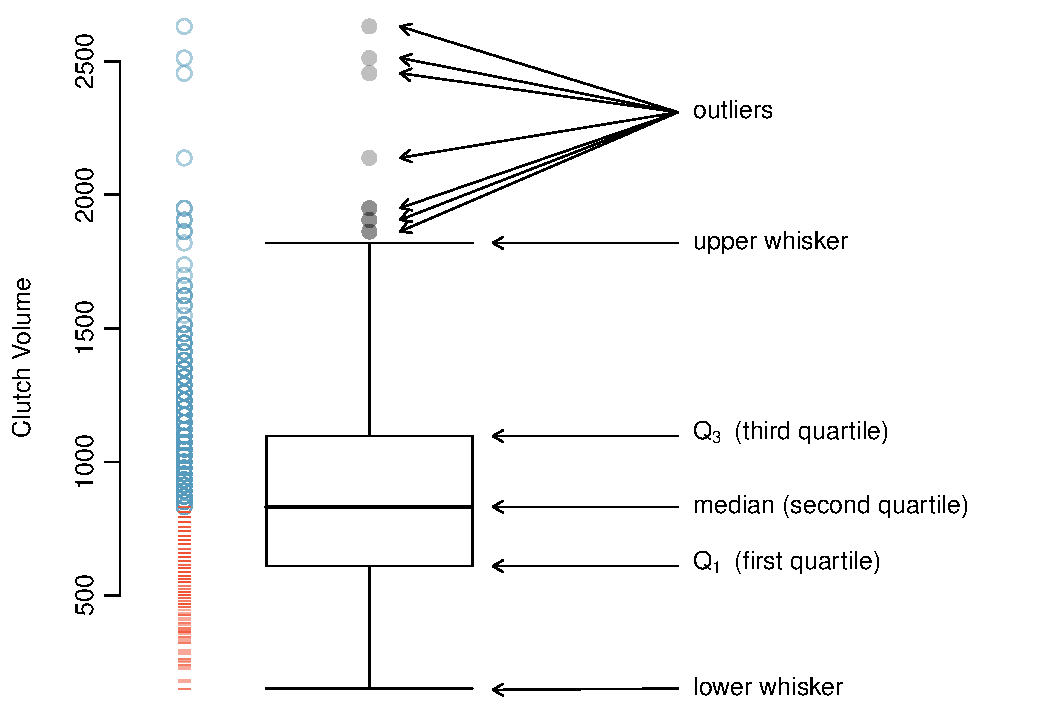
\includegraphics[width=\maxwidth]{figure/unnamed-chunk-1-1} 

}

\caption{A boxplot and dot plot of \texttt{clutch.volume} in the \texttt{frog} dataset from the \texttt{oibiostat} package. The horizontal dashes indicate the bottom 50\% of the data and the open circles represent the top 50\%.}\label{fig:unnamed-chunk-1}
\end{figure}

\end{knitrout}
		\end{column}
		\begin{column}{0.5\textwidth}
			\begin{itemize}
				\item We previously examined the variability in data. 
				\item In the statistical context, data is obtained by selecting a sample from the
				target population and measuring the quantities of interest for the
				subjects that belong to the sample. 
				\item Different subjects in the sample may obtain different values for the measurement, leading to variability in
				the data.
				\item Numerical summaries may be computed in order to characterize the main
				features of the variability, e.g., mean, median, sample variance, sample standard deviation, inter-quartile range
			\end{itemize}
		\end{column}
	\end{columns}
\end{frame}



\begin{frame}{Two other forms of variability}
	
	\begin{itemize}
		
		\item  The subject of this section is to introduce two other forms of
		variability, variability that is not associated, at least not directly,
		with the data that we observe. \pause
		\begin{enumerate}
			\item Population variability
			\item Variability of a random variable
		\end{enumerate}

	\pause
		
		\item The notions of variability that will be presented are abstract, they are
		not given in terms of the data that we observe, and they have a
		mathematical-theoretical flavor to them. 
		
		\pause
		
		\item At first, these abstract
		notions may look to you as a waste of your time and may seem to be
		unrelated to the subject matter of the course. 
		
		\pause
		
		\item The opposite is true. The
		very core of statistical thinking is relating observed data to
		theoretical and abstract models of a phenomena. 
		
		\pause 
		\item The abstract notions of variability that are introduced in this
		chapter, and are extended in the subsequent chapters, are the essential foundations for the practice of
		statistics
	\end{itemize}
	
\end{frame}


\begin{frame}{Population variability}
	
	\begin{itemize}[<+->]
		
		\item  We will examine the data set \texttt{heights\_sample.csv} available at \url{https://github.com/sahirbhatnagar/EPIB607/blob/master/inst/data/heights_sample.csv} which contains data on the sex and height of a sample of 100 observations. 
		\item We will also consider the sex and height of all the members of the population from which the sample was selected available at \url{https://github.com/sahirbhatnagar/EPIB607/blob/master/inst/data/heights_population.csv}
		\item The size of the relevant population is 100,000, including the 100
		subjects that composed the sample. 
		\item When we examine the values of the
		height across the entire population we can see that different people may
		have different heights. This variability of the heights is the \textbf{population variability}
	\end{itemize}
	
\end{frame}


\begin{frame}{Variability of a random variable}
	
	\begin{itemize}[<+->]
		
		\item  The other abstract type of variability, the \textbf{variability of a random variable}, is a mathematical concept. 
		\item The aim of this concept is to model the notion of randomness in measurements or the uncertainty regarding
		the outcome of a measurement. 
		\item In particular we will initially consider the variability of a random variable in the context of selecting one
		subject at random from the population.
		\item Random variables provide models for randomness and uncertainty in measurements. 
		\item Simple examples of such abstract random variables will be provided in this
		chapter. More examples will be introduced in the subsequent chapters.
	\end{itemize}
	
\end{frame}


\begin{frame}{A point to remember}
	
	\begin{itemize}[<+->]
		
		\item The variability of the data relates to a concrete list of data values that is presented to us. 
		\item The other types of variability are
		not associated with quantities we actually get to observe. 
		\item  The data for
		the sample we get to see but not the data for the rest of the
		population. 
		\item Yet, we can still discuss the variability of a population
		that is out there, even though we do not observe the list of
		measurements for the entire population. 
		\item The discussion of the variability in this context
		is theoretical in its nature. Still, this theoretical discussion is
		instrumental for understanding statistics.
	\end{itemize}
	
\end{frame}



\section{Variability of a population}


\begin{frame}[fragile]{Sample of heights}

\begin{knitrout}\scriptsize
\definecolor{shadecolor}{rgb}{0.969, 0.969, 0.969}\color{fgcolor}\begin{kframe}
\begin{alltt}
\hlkwd{library}\hlstd{(dplyr)}
\hlkwd{library}\hlstd{(rio)}

\hlstd{heights_sample} \hlkwb{<-} \hlstd{rio}\hlopt{::}\hlkwd{import}\hlstd{(}
                   \hlstd{here}\hlopt{::}\hlkwd{here}\hlstd{(}\hlstr{"inst/data/heights_sample.csv"}\hlstd{))}
\hlstd{heights_sample} \hlkwb{<-} \hlstd{heights_sample} \hlopt
                    \hlstd{dplyr}\hlopt{::}\hlkwd{mutate}\hlstd{(}\hlkwc{sex} \hlstd{=} \hlkwd{factor}\hlstd{(sex))}

\hlkwd{summary}\hlstd{(heights_sample)}
\end{alltt}
\begin{verbatim}
##        id              sex         height     
##  Min.   :1538611   FEMALE:54   Min.   :117.0  
##  1st Qu.:3339583   MALE  :46   1st Qu.:158.0  
##  Median :5105620               Median :171.0  
##  Mean   :5412367               Mean   :170.1  
##  3rd Qu.:7622236               3rd Qu.:180.2  
##  Max.   :9878130               Max.   :208.0
\end{verbatim}
\begin{alltt}
\hlstd{heights_sample} \hlopt
   \hlstd{dplyr}\hlopt{::}\hlkwd{glimpse}\hlstd{()}
\end{alltt}
\begin{verbatim}
## Rows: 100
## Columns: 3
## $ id     <int> 5696379, 3019088, 2038883, 1920587, 6006813, 4055945, 9263269, ~
## $ sex    <fct> FEMALE, MALE, MALE, FEMALE, MALE, FEMALE, FEMALE, FEMALE, MALE,~
## $ height <int> 182, 168, 172, 154, 174, 176, 193, 156, 157, 186, 143, 182, 194~
\end{verbatim}
\end{kframe}
\end{knitrout}

\end{frame}


\begin{frame}[fragile]{Population of heights}
	
\begin{knitrout}\scriptsize
\definecolor{shadecolor}{rgb}{0.969, 0.969, 0.969}\color{fgcolor}\begin{kframe}
\begin{alltt}
\hlstd{heights_population} \hlkwb{<-} \hlstd{rio}\hlopt{::}\hlkwd{import}\hlstd{(}
                 \hlstd{here}\hlopt{::}\hlkwd{here}\hlstd{(}\hlstr{"inst/data/heights_population.csv"}\hlstd{))}
\hlstd{heights_population} \hlkwb{<-} \hlstd{heights_population} \hlopt
                    \hlstd{dplyr}\hlopt{::}\hlkwd{mutate}\hlstd{(}\hlkwc{sex} \hlstd{=} \hlkwd{factor}\hlstd{(sex))}

\hlkwd{summary}\hlstd{(heights_population)}
\end{alltt}
\begin{verbatim}
##        id              sex            height   
##  Min.   :1000082   FEMALE:48888   Min.   :117  
##  1st Qu.:3254220   MALE  :51112   1st Qu.:162  
##  Median :5502618                  Median :170  
##  Mean   :5502428                  Mean   :170  
##  3rd Qu.:7757518                  3rd Qu.:178  
##  Max.   :9999937                  Max.   :217
\end{verbatim}
\begin{alltt}
\hlstd{heights_population} \hlopt
   \hlstd{dplyr}\hlopt{::}\hlkwd{glimpse}\hlstd{()}
\end{alltt}
\begin{verbatim}
## Rows: 100,000
## Columns: 3
## $ id     <int> 5696379, 3019088, 2038883, 1920587, 6006813, 4055945, 9263269, ~
## $ sex    <fct> FEMALE, MALE, MALE, FEMALE, MALE, FEMALE, FEMALE, FEMALE, MALE,~
## $ height <int> 182, 168, 172, 154, 174, 176, 193, 156, 157, 186, 143, 182, 194~
\end{verbatim}
\end{kframe}
\end{knitrout}
	
\end{frame}


\begin{frame}[fragile]{Distribution of population of heights}
	
\begin{knitrout}\scriptsize
\definecolor{shadecolor}{rgb}{0.969, 0.969, 0.969}\color{fgcolor}\begin{kframe}
\begin{alltt}
\hlkwd{library}\hlstd{(ggplot2);} \hlkwd{library}\hlstd{(cowplot)}
\hlstd{ggplot2}\hlopt{::}\hlkwd{theme_set}\hlstd{(cowplot}\hlopt{::}\hlkwd{theme_cowplot}\hlstd{())}
\hlstd{p} \hlkwb{<-} \hlkwd{ggplot}\hlstd{(}\hlkwc{data} \hlstd{= heights_population,}
             \hlkwc{mapping} \hlstd{=} \hlkwd{aes}\hlstd{(}\hlkwc{x} \hlstd{= height))}
\hlstd{p} \hlopt{+} \hlkwd{geom_bar}\hlstd{()}
\end{alltt}
\end{kframe}

{\centering 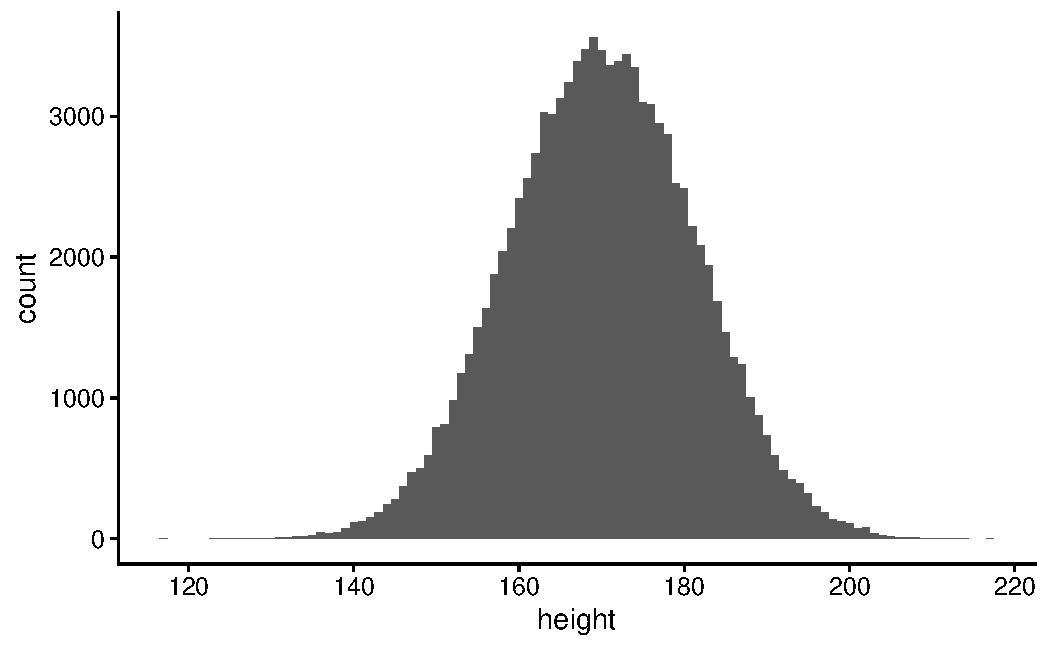
\includegraphics[width=\maxwidth]{figure/unnamed-chunk-4-1} 

}


\end{knitrout}
	
\end{frame}



\begin{frame}{Population mean $\mu$}
	
	\begin{itemize}[<+->]
		
		\item The formula of the population mean is:
		
		$$\mu = \frac{\mbox{Sum of all values in the population}}{\mbox{Number of values in the population}}= \frac{\sum_{i=1}^N y_i}{N}\;.$$
		
		
		\item Observe the similarity between the definition of the mean for the data
		and the definition of the mean for the population. In both cases the
		arithmetic average is computed. The only difference is that in the case
		of the mean of the data the computation is with respect to the values
		that appear in the sample whereas for the population all the values in
		the population participate in the computation.
		
		\item In actual life, we will not have all the values of a variable in the
		entire population. Hence, we will not be able to compute the actual
		value of the population mean. 
		
		\item It's still meaningful to talk about the population mean because this number exists, even though we do
		not know what its value is. Statistics is about trying to estimate this unknown quantity on the basis of the data we do have in the sample.
		
	\end{itemize}
	
\end{frame}


\begin{frame}[fragile]{Population variance $\sigma^2$}
	
	\begin{itemize}[<+->]
		
		\item The formula of the population variance is defined in a similar way:
		
$$
\begin{aligned}
	\sigma^2 =& \mbox{The average square deviation in the population}\\
	=& \frac{\mbox{Sum of the squares of the deviations in the population}}{\mbox{Number of values in the population}}\\
	=& \frac{\sum_{i=1}^N (y_i-\mu)^2}{N}\;.
\end{aligned}
$$
		
		\item In \texttt{R}:
		
\begin{knitrout}\scriptsize
\definecolor{shadecolor}{rgb}{0.969, 0.969, 0.969}\color{fgcolor}\begin{kframe}
\begin{alltt}
\hlstd{N} \hlkwb{<-} \hlkwd{nrow}\hlstd{(heights_population)}
\hlkwd{var}\hlstd{(heights_population}\hlopt{$}\hlstd{height)} \hlopt{*} \hlstd{(N} \hlopt{-} \hlnum{1}\hlstd{)} \hlopt{/} \hlstd{N}
\end{alltt}
\begin{verbatim}
## [1] 126.1576
\end{verbatim}
\end{kframe}
\end{knitrout}
		
		\item The standard deviation of the population, yet another parameter, is
		denoted by $\sigma$ and is equal to the square root of the variance. 
		
		\item The typical situation is that we do not
		know what the actual value of $\sigma$. Yet, we may refer to it as a quantity and we may try to estimate its
		value based on the data we do have from the sample.
		
		

		
	\end{itemize}
	
\end{frame}


\section{Variability of a random variable}


\begin{frame}[fragile]{Variability of a random variable}
	
	\begin{itemize}[<+->]
		
		\item As an example, consider taking a sample of size $n=1$ from the population (a single
		person) and measuring his/her height. We will apply the function \texttt{dplyr::sample\_n} to sample one row from the data frame:
		
\begin{knitrout}\tiny
\definecolor{shadecolor}{rgb}{0.969, 0.969, 0.969}\color{fgcolor}\begin{kframe}
\begin{alltt}
\hlstd{heights_population} \hlopt
   \hlstd{dplyr}\hlopt{::}\hlkwd{sample_n}\hlstd{(}\hlkwc{size} \hlstd{=} \hlnum{1}\hlstd{)}
\end{alltt}
\begin{verbatim}
##        id  sex height
## 1 2513465 MALE    170
\end{verbatim}
\end{kframe}
\end{knitrout}
		
		\item Let us run the function again:
		
\begin{knitrout}\tiny
\definecolor{shadecolor}{rgb}{0.969, 0.969, 0.969}\color{fgcolor}\begin{kframe}
\begin{alltt}
\hlstd{heights_population} \hlopt
\hlstd{dplyr}\hlopt{::}\hlkwd{sample_n}\hlstd{(}\hlkwc{size} \hlstd{=} \hlnum{1}\hlstd{)}
\end{alltt}
\begin{verbatim}
##        id  sex height
## 1 5178027 MALE    159
\end{verbatim}
\end{kframe}
\end{knitrout}

\item And again

\begin{knitrout}\tiny
\definecolor{shadecolor}{rgb}{0.969, 0.969, 0.969}\color{fgcolor}\begin{kframe}
\begin{alltt}
\hlstd{heights_population} \hlopt
\hlstd{dplyr}\hlopt{::}\hlkwd{sample_n}\hlstd{(}\hlkwc{size} \hlstd{=} \hlnum{1}\hlstd{)}
\end{alltt}
\begin{verbatim}
##        id  sex height
## 1 1006901 MALE    174
\end{verbatim}
\end{kframe}
\end{knitrout}
		
		
	\end{itemize}
	
\end{frame}


\begin{frame}[fragile]{Random variable}
	\small
	\begin{itemize}[<+->]
		
		\item A random variable is the future outcome of a measurement, \textbf{before}
		the measurement is taken. It does not have a specific value, but rather
		a collection of potential values with a distribution over these values.
		
		\item After the measurement is taken and the specific value is revealed then
		the random variable ceases to be a random variable! Instead, it becomes
		data.
		
		\item One is not able to say what the outcome of a random variable
		will turn out to be. 
		
		\item However, one may identify patterns in this potential
		outcome. For example, knowing that the distribution of heights in the
		population ranges between 117 and 217 centimeter one may say in advance
		that the outcome of the measurement must also be in that interval.
		
		\item Since there is a total of 3,476 subjects with height equal to
		168 centimeters and since the likelihood of each subject to be selected
		is equal then the likelihood of selecting a subject of this height is
		3,476/100,000 = 0.03476. In the context of random variables we call this
		likelihood probability. 
		
		\item In the same vain, the frequency of subjects
		with hight 192 centimeter is 488, and therefore the probability of
		measuring such a height is 0.00488. The frequency of subjects with
		height 200 centimeter or above is 393, hence the probability of
		obtaining a measurement in the range between 200 and 217 centimeter is
		0.00393.
		
		
	\end{itemize}
	
\end{frame}


\begin{frame}[fragile]{Sample Space and Distribution}
	\small
	\begin{itemize}[<+->]
		
		\item A random variable refer to numerical values, typically the outcome of an
		observation, a measurement, or a function thereof.
		
		\item A random variable is characterized via the collection of potential
		values it may obtain, known as the \textbf{sample space} and the likelihood of
		obtaining each of the values in the sample space (namely, the
		probability of the value).
		
		\item The probability of each value is the height
		of the bar above the value, divided by the total frequency of 100,000
		(namely, the relative frequency in the population).
		
		\item We will denote random variables with capital Latin letters such as $X$,
		$Y$, and $Z$. Values they may obtain will be marked by small Latin
		letters such as $x$, $y$, $z$. For the probability of values we will use
		the letter “$\Prob$". Hence, if we denote by $Y$ the measurement of
		height of a random individual that is sampled from the given population
		then: 
		
		$$\Prob(Y = 168) = 0.03476$$ and 
		$$\Prob(Y \geq 200) = 0.00393\;.$$
		
	\end{itemize}
	
\end{frame}



\begin{frame}[fragile]{Sample Space and Distribution}
	\small
	\begin{itemize}[<+->]
		
		\item Consider, as yet another example, the probability that the height of a
		random person sampled from the population differs from 170 centimeter by
		no more than 10 centimeters. (In other words, that the height is between
		160 and 180 centimeters.) Denote by $Y$ the height of that random
		person. We are interested in the probability
		$\Prob(|Y -170| \leq 10)$
		
		\item In \texttt{R}:
		
\begin{knitrout}
\definecolor{shadecolor}{rgb}{0.969, 0.969, 0.969}\color{fgcolor}\begin{kframe}
\begin{alltt}
\hlstd{Y} \hlkwb{<-} \hlstd{heights_population}\hlopt{$}\hlstd{height}

\hlkwd{mean}\hlstd{(}\hlkwd{abs}\hlstd{(Y}\hlopt{-}\hlnum{170}\hlstd{)} \hlopt{<=} \hlnum{10}\hlstd{)}
\end{alltt}
\begin{verbatim}
## [1] 0.64541
\end{verbatim}
\end{kframe}
\end{knitrout}
		
	\end{itemize}
	
\end{frame}



\begin{frame}[fragile]{A note on the previous calculation}
	\small
	\begin{itemize}[<+->]
		
		\item Let us produce a small example that will help us explain the computation
		of the probability. We start by forming a sequence with 10 numbers:
				
\begin{knitrout}
\definecolor{shadecolor}{rgb}{0.969, 0.969, 0.969}\color{fgcolor}\begin{kframe}
\begin{alltt}
\hlstd{Y} \hlkwb{<-} \hlkwd{c}\hlstd{(}\hlnum{6.3}\hlstd{,} \hlnum{6.9}\hlstd{,} \hlnum{6.6}\hlstd{,} \hlnum{3.4}\hlstd{,} \hlnum{5.5}\hlstd{,} \hlnum{4.3}\hlstd{,} \hlnum{6.5}\hlstd{,} \hlnum{4.7}\hlstd{,} \hlnum{6.1}\hlstd{,} \hlnum{5.3}\hlstd{)}
\end{alltt}
\end{kframe}
\end{knitrout}
		
		The goal is to compute the proportion of numbers that are in the range
		$[4,6]$ (or, equivalently, $\{|Y-5| \leq 1\}$).
		
		\item 
		
\begin{knitrout}
\definecolor{shadecolor}{rgb}{0.969, 0.969, 0.969}\color{fgcolor}\begin{kframe}
\begin{alltt}
\hlkwd{abs}\hlstd{(Y}\hlopt{-}\hlnum{5}\hlstd{)}
\end{alltt}
\begin{verbatim}
##  [1] 1.3 1.9 1.6 1.6 0.5 0.7 1.5 0.3 1.1 0.3
\end{verbatim}
\end{kframe}
\end{knitrout}

\item 

\begin{knitrout}
\definecolor{shadecolor}{rgb}{0.969, 0.969, 0.969}\color{fgcolor}\begin{kframe}
\begin{alltt}
\hlkwd{abs}\hlstd{(Y} \hlopt{-} \hlnum{5}\hlstd{)} \hlopt{<=} \hlnum{1}
\end{alltt}
\begin{verbatim}
##  [1] FALSE FALSE FALSE FALSE  TRUE  TRUE FALSE  TRUE FALSE  TRUE
\end{verbatim}
\end{kframe}
\end{knitrout}


\item 		
\begin{knitrout}
\definecolor{shadecolor}{rgb}{0.969, 0.969, 0.969}\color{fgcolor}\begin{kframe}
\begin{alltt}
\hlkwd{mean}\hlstd{(}\hlkwd{abs}\hlstd{(Y} \hlopt{-} \hlnum{5}\hlstd{)} \hlopt{<=} \hlnum{1}\hlstd{)}
\end{alltt}
\begin{verbatim}
## [1] 0.4
\end{verbatim}
\end{kframe}
\end{knitrout}
		
	\end{itemize}
	
\end{frame}




\begin{frame}[fragile]{Probability function}
	\small
	\begin{itemize}[<+->]
		
		\item The probability function of a random variable is defined for any value
		that the random variable may obtain and produces the \textbf{distribution} of
		the random variable. The probability function may emerge as a relative
		frequency as in the given example or it may be a result of theoretical
		modeling.
		
		\item Consider the following probability distribution:
		
\begin{knitrout}\small
\definecolor{shadecolor}{rgb}{0.969, 0.969, 0.969}\color{fgcolor}
\begin{tabular}{rrr}
\toprule
Value & Probability & Cum.Prob\\
\midrule
0 & 0.50 & 0.50\\
1 & 0.25 & 0.75\\
2 & 0.15 & 0.90\\
3 & 0.10 & 1.00\\
\bottomrule
\end{tabular}

\end{knitrout}
		
		\item What is $\Prob(Y=0)$, the probability that $Y$ is equal to 0?:
		
		\item What is the probability of $Y$ falling in the interval $[0.5, 2.3]$ ?
		
		
	\end{itemize}
	
\end{frame}



\begin{frame}[fragile]{Expectation}
	\small
	\begin{itemize}[<+->]
		
		\item We may characterize the center of the distribution of a random variable
		and the spread of the distribution in ways similar to those used for the
		characterization of the distribution of data and the distribution of a
		population.
		
		\item The \textbf{expectation} marks the center of the distribution of a random
		variable. It is equivalent to the data average $\bar y$ and the
		population average $\mu$, which was used in order to mark the location
		of the distribution of the data and the population, respectively.
		

	\end{itemize}
	
\end{frame}



\begin{frame}[fragile]{Expectation}
	\small
	\begin{itemize}[<+->]
		
		\item The average of the data can be computed as the weighted average of the values that are present
		in the data, with weights given by the relative frequency. Specifically,
		for the data
		
		$$1,\; 1,\; 1,\; 2,\; 2,\; 3,\; 4,\; 4,\; 4,\; 4,\; 4,$$ the mean can be calculated via
		
		\begin{align*}
			\bar{y} &= \frac{1 + 1 + 1 + 2 + 2 + 3 + 4 + 4 + 4 + 4 + 4}{11}\\
			& =	1\times \frac{3}{11} + 2 \times \frac{2}{11} + 3 \times \frac{1}{11} + 4 \times \frac{5}{11}
		\end{align*}

		producing the value of $\bar y =2.727$ in both representations. 
		
		\item Using a formula, the equality between the two ways of computing the mean is
		given in terms of the equation:
		
		$$\bar y = \frac{\sum_{i=1}^n y_i}{n} = \sum_y \big(y \times (f_y/n)\big)\;,$$
		where $f_y$ represents the frequency of $y$ in the data. 
		

		
		
	\end{itemize}
	
\end{frame}


\begin{frame}[fragile]{Expectation}
	\small
	\begin{itemize}		
	
		\item Using a formula, the equality between the two ways of computing the mean is
		given in terms of the equation:
		
		$$\bar y = \frac{\sum_{i=1}^n y_i}{n} = \sum_y \big(y \times (f_y/n)\big)\;,$$
		where $f_y$ represents the frequency of $y$ in the data. 
		
		\item The expectation of a random variable is computed in the spirit of the
		second formulation, and is define via the equation:
		
		$$\Expec(Y) = \sum_y \big(y \times \Prob(y)\big)\;.$$
		
		
	\end{itemize}
	
\end{frame}



\begin{frame}[fragile]{Variance}
	\small
	\begin{itemize}		
		
		\item The sample variance ($s^2$) is obtained as the sum of the squared
		deviations from the average, divided by the sample size ($n$) minus 1:
		
		$$s^2 = \frac{\sum_{i=1}^n (y_i - \bar y)^2}{n-1}\;.$$ 
		
		\item  A second	formulation for the computation of the same quantity is via the use of
		relative frequencies. The formula for the sample variance takes the form
		
		$$s^2 = \frac{n}{n-1}\sum_y \big((y - \bar y)^2\times (f_y/n)\big)\;.$$
		
		
		\item In a similar way, the variance of a random variable may be defined via
		the deviation from the expectation. This deviation is
		then squared and multiplied by the probability of the value. The
		multiplications are summed up in order to produce the variance:
		
		$$\Var(Y) = \sum_y\big( (y-\Expec(Y))^2 \times \Prob(y)\big)\;.$$
		
	\end{itemize}
	
\end{frame}


	\begin{frame}[fragile]{Session Info}
	\tiny
	
\begin{knitrout}\tiny
\definecolor{shadecolor}{rgb}{0.969, 0.969, 0.969}\color{fgcolor}\begin{kframe}
\begin{verbatim}
R version 4.0.4 (2021-02-15)
Platform: x86_64-pc-linux-gnu (64-bit)
Running under: Pop!_OS 21.04

Matrix products: default
BLAS:   /usr/lib/x86_64-linux-gnu/openblas-pthread/libblas.so.3
LAPACK: /usr/lib/x86_64-linux-gnu/openblas-pthread/libopenblasp-r0.3.13.so

attached base packages:
[1] tools     stats     graphics  grDevices utils     datasets  methods  
[8] base     

other attached packages:
 [1] cowplot_1.1.0       rio_0.5.16          openintro_2.2.0    
 [4] usdata_0.1.0        cherryblossom_0.1.0 airports_0.1.0     
 [7] oibiostat_0.2.0     DT_0.16             kableExtra_1.2.1   
[10] socviz_1.2          gapminder_0.3.0     here_0.1           
[13] NCStats_0.4.7       FSA_0.8.30          forcats_0.5.1      
[16] stringr_1.4.0       dplyr_1.0.7         purrr_0.3.4        
[19] readr_1.4.0         tidyr_1.1.3         tibble_3.1.3       
[22] ggplot2_3.3.5       tidyverse_1.3.0     knitr_1.33         

loaded via a namespace (and not attached):
 [1] fs_1.5.0           lubridate_1.7.9    webshot_0.5.2      httr_1.4.2        
 [5] rprojroot_2.0.2    backports_1.2.1    utf8_1.2.2         R6_2.5.1          
 [9] DBI_1.1.1          colorspace_2.0-2   withr_2.4.2        tidyselect_1.1.1  
[13] gridExtra_2.3      leaflet_2.0.3      curl_4.3.2         compiler_4.0.4    
[17] cli_3.0.1          rvest_1.0.0        pacman_0.5.1       xml2_1.3.2        
[21] ggdendro_0.1.22    labeling_0.4.2     mosaicCore_0.8.0   scales_1.1.1      
[25] digest_0.6.27      ggformula_0.9.4    foreign_0.8-81     rmarkdown_2.9.7   
[29] pkgconfig_2.0.3    htmltools_0.5.2    highr_0.9          dbplyr_1.4.4      
[33] fastmap_1.1.0      htmlwidgets_1.5.3  rlang_0.4.11       readxl_1.3.1      
[37] rstudioapi_0.13    farver_2.1.0       generics_0.1.0     jsonlite_1.7.2    
[41] crosstalk_1.1.1    zip_2.2.0          car_3.0-9          magrittr_2.0.1    
[45] mosaicData_0.20.1  Matrix_1.3-2       Rcpp_1.0.7         munsell_0.5.0     
[49] fansi_0.5.0        abind_1.4-5        lifecycle_1.0.0    stringi_1.7.3     
[53] carData_3.0-4      MASS_7.3-53.1      plyr_1.8.6         ggstance_0.3.4    
[57] grid_4.0.4         blob_1.2.1         ggrepel_0.8.2      crayon_1.4.1      
[61] lattice_0.20-41    haven_2.3.1        splines_4.0.4      hms_1.0.0         
[65] pillar_1.6.2       reprex_0.3.0       glue_1.4.2         evaluate_0.14     
[69] data.table_1.14.0  modelr_0.1.8       vctrs_0.3.8        tweenr_1.0.1      
[73] cellranger_1.1.0   gtable_0.3.0       polyclip_1.10-0    assertthat_0.2.1  
[77] TeachingDemos_2.12 xfun_0.25          ggforce_0.3.2      openxlsx_4.1.5    
[81] broom_0.7.2        viridisLite_0.4.0  mosaic_1.7.0       ellipsis_0.3.2    
\end{verbatim}
\end{kframe}
\end{knitrout}
	
\end{frame}

\end{document}

































\begin{frame}{The (statistical) parameters we will be concerned with: $\mu$}
	

\begin{itemize}
	\item $\mu$: The mean level of a quantitative characteristic, e.g. the depth of the earth's ocean or height of the land, or the height / BMI / blood pressure levels of a human population. \pause 
	\item One could also think of mathematical and physical constants as parameters, even though their values are effectively 'known.' Examples where there is agreement to many many decimal places include the mathematical constant pi, the speed of light (c), and the gravitational constant G. The speed of sound depends on the medium it is travelling through, and the temperature of the medium. The freezing and boiling points of substances such as water and milk depend on altitude and barometric pressure.  \pause 
	\item At a lower level, we might be interested in personal characters, such as the size of a person's vocabulary, or a person's mean (or minimum, or typical) reaction time. The  target could be a person's 'true score' on some test -- the  value one would get if one (could, but not realistically) be tested on each of the (very large) number of test items in the test bank, or observed/measured continously over the period of interest.  

\end{itemize}

\end{frame}



\begin{frame}{The (statistical) parameters we will be concerned with: $\pi$}
	
	
	\begin{itemize}
	
		\item $\pi$: Prevalence or risk (proportion): e.g.,  proportion of the earth's surface that is covered by water, or of a human population that has untreated hypertension, or lacks internet access, or will develop a new health condition over the next x years. \pause 
		\item At a lower level, we might be interested in personal proportions, such as what proportion of the calories a person consumes come from fat, or the proportion of the year 2020 the person spent on the internet, or indoors, or asleep, or sedentary.	
	\end{itemize}
	
\end{frame}





\begin{frame}{The (statistical) parameters we will be concerned with: $\lambda$}
	
	
	\begin{itemize}
			
		\item $\lambda$: The speed with which events occur: e.g., earthquakes per earth-day, or heart attacks or traffic fatalities per (population)-year. 
		\item At a lower level, we might be interested in personal intensities, such as the mean number of tweets/waking-hour  a person issued during the year 2020, or the mean number of times per 100 hours of use a person's laptop froze and needed to be re-booted.
		
	\end{itemize}
	
\end{frame}



\begin{frame}{The (statistical) parameters we will be concerned with}
	
	
	\begin{itemize}
		\item Each of these three parameters refers to a characteristic of the overall domain, such as entire surface of the earth, or the entire ocean, or population. There are no indicators for distinguishing among subdomains, so they refer to locations / persons not otherwise specified. We will drill down  later. \pause 
		
		\item Especially for epidemiologic research, and also more generally, one can think  of $\pi$ and $\lambda$ as  parameters of occurrence. [Although the word occurrence usually has a time element, it can also be timeless: how frequently a word occurs in a static text, or a mineral in a rock.] \pause 
		
		\item Prevalence is the proportion in a current state, and the 5-year risk is the expected proportion or probability of being in a new state 5 years from now. The  parameter $\lambda$ measures the speed with which the  elements in question move from the original to the other state.\pause 
		
		\item Even though the depths of the ocean, and blood pressures, are measured on a quantitative (rather than on all or none) scale, one can divide the scale into a finite number of bins/caterories, and speak of the prevalence (proportion) in each category. Conversely, one can use a set of descriptive parameters called quantiles, i.e, landmarks such that selected proportions, e.g., 0.05 or 5\%, 25\%, 50\%, 75\%, 95\% of the distribution are to the left of ('below') these quantiles.
	\end{itemize}
	
\end{frame}



\begin{frame}{Terminology}
\begin{itemize}
	\item Before we go on, we need to adopt sensible terminology for referring generically to the states, traits, conditions or behaviours  whose category-specific parameter values are being compared. \pause 
	
	\item We will use the term  \textbf{determinant}. It has several advantages over the many other terms used in different disciplines, such as exposure, agent, independent/explanatory variable, experimental condition, treatment, intervention, factor, risk factor, predictor. The main advantage is that it is broader, and closer to causally neutral in its connotaion. \pause 
	
	\item  \textit{Exposure} has environmental connotations, and technically refers to an opportity to injest or mentally take on board a substance or message.  
	\pause 
	\item The term \textit{independent variable} suggests the investigator has control over it in a laboratory setting. 
	\pause 
	\item The term \textit{explanatory} is  ambiguous as to the mechanism by which the parameter value in the index category got to be different from the value in the index category. Not all contrasts are experimentally formed. 

\end{itemize}
\end{frame}


\begin{frame}{Terminology}
	\begin{itemize}
		\item The term \textit{factor}, and thus the term \textit{risk factor}, are to be avoided because the word factor derives from the Latin \textit{facere}, (the action of) doing, making, creating. 
		\pause 		
		\item \textit{Predictor} makes one think of the future. 
		
		\pause 
		\item The term \textit{regressor} (or its shorthand, the 'X' ) won't be understood by lay people.
		
				\pause 
		\item While the word \textbf{determine} can suggest causality (e.g., demand determines the price), it also refers to 'fixing the form, position, or character of beforehand': two points determine a straight line; the area of a circle is determined by its radius.
		
				\pause 
		\item We now move on to the parameter relations we will be concerned with, beginning with the simplest type.
	\end{itemize}
\end{frame}



\begin{frame}{Parameter Contrasts}
	\begin{itemize}
		\item In applied research, we are seldom interested in a single constant. 
		
		
				\pause 
		
		\item Much more often we are interested in the contrast (difference) between the parameter values in different contexts/locations (Northern hemisphere vs Southern hemisphere), conditions/times (reaction times using the right versus left hand, or behaviour on weekdays versus weekends), or sub-domains or sub-populations (females vs males).
		
		\pause 
		
		\item In this section, we will limit our attention to 'contrasts': a compariosn of the parameter values between 2 contexts/locations/sub-populations. Thus the parameter function has just 2 possible 'input' values. 
	\end{itemize}
\end{frame}



\begin{frame}{'Reference' and 'Index' categories}
	\begin{itemize}
		\item In many research contexts, the choice of 'reference' category (starting point, the category against which the other category is compared) will be obvious: it is the \textbf{status quo} (standard care, prevailing condition or usual situation, dominant hand, better known category). 
		\pause 
		\item The 'index' category is \textbf{the category one is curious about} and wishes to learn more about, by contrasting its parameter value with the parameter value for the reference category.
		\pause 		
		\item In other contexts, it is less obvious which category should serve as the reference and the index categories, and the choice may be merely a matter of persepctive. If one is more famiar with the Northern hemisphere, it serves as a natural starting point 
		
				\pause 
		\item The choice of reference category in a longevity contrast between males and females, or in-hospital mortality rates or motor vehicle fatality rates during weekends versus weekdays, might depend on what mechanism one wishes to bring out. 
		
				\pause 
		\item Or one might chose as the reference category the one with the larger amount of experience, or maybe the one with the lower parameter value, so that the 'index minus reference' difference would be a positive quantity, or the 'index: reference ratio' exceeds 1.
	\end{itemize}
\end{frame}




\begin{frame}{'Reference' and 'Index' categories}
	\begin{itemize}
		\item The choice of reference category in a longevity contrast between males and females, or in-hospital mortality rates or motor vehicle fatality rates during weekends versus weekdays, might depend on what mechanism one wishes to bring out. 
		
		\item Or one might chose as the reference category the one with the larger amount of experience, or maybe the one with the lower parameter value, so that the 'index minus reference' difference would be a positive quantity, or the 'index: reference ratio' exceeds 1.
	\end{itemize}
\end{frame}



\begin{frame}{Parameter relations in numbers and words}
\begin{itemize}
\item To make this concrete, we will use hypothetical (and very round) numbers and pretend we 'know' the true parameter values -- in our example
of the mean depth of the ocean in the Northern hemisphere (reference category) and Southern hemisphere (index category) -- to be 3,600 metres (3.6Km) and 4,500 metres (4.5Km) respectively. Thus, the difference (South minus North) is 900 metres or 0.9Km.
\pause
\item If we wished to show the two parameter values graphically, we might do so using the format in panel (a), which shows the 2 hemisphere-specific parameter values -- but forces the reader to calculate the difference.

\item Panel (b) follows a more reader-friendy format, where the difference (the quantity of interest) is isolated:  the original 2 parameters are converted to 2 new, more relevant ones. 

\item Panel (c) encodes the relation displayed in panel (b) in a \textbf{single phrase} that applies to \textbf{both} categories: Onto the 'starting value' of 3.8Km, one \textbf{adds} $\Delta \mu$ = 0.9 Km \textbf{only if} the  resulting parameter pertains to the Southern hemisphere. The 0.9 Km is toggled off/on as one moves from North to South.   
\end{itemize}
\end{frame}




\begin{frame}[fragile,plain]

\begin{knitrout}\tiny
\definecolor{shadecolor}{rgb}{0.969, 0.969, 0.969}\color{fgcolor}

{\centering 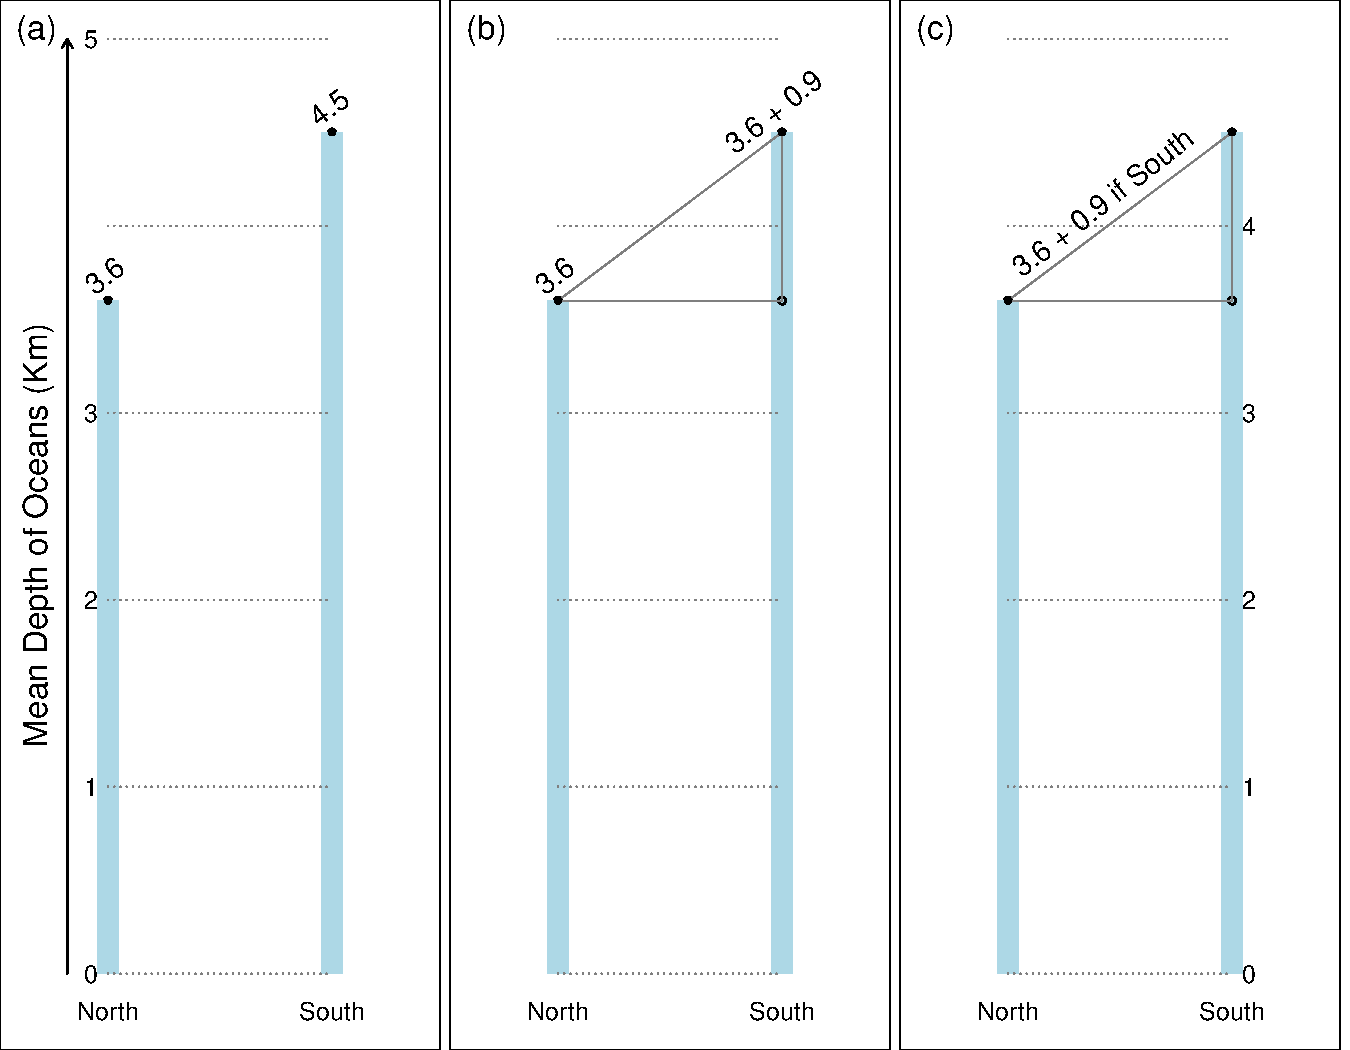
\includegraphics[width=\maxwidth]{figure/unnamed-chunk-16-1} 

}


\end{knitrout}
\end{frame}


\begin{frame}{Parameter relations in symbols, and with the help of an  index-category indicator}
\begin{itemize}
\item Panels (a) and (b) in the following figure repeat the information in panels (a) and (b) in the preceding Figure, but using Greek letters to symbolically represent the parameters. Just to keep the graphics uncluttered, the labels North and South are abbreviated to N and S and used as subscripts. Also, for brevity, the expression $\Delta \mu$ denotes $\mu_S - \mu_N$. 

\pause 

\item The relation encoded in a single phrase shown in the previous panel (c) has a compact form suitable for verbal communication. The representation can be adapted to be more suitable for computer calculations. (The benefit of doing this will become obvious as soon as you try to learn the parameter values by fiiting these models to actual data.) Depending on whether the hemisphere in question is the northern or southern hemisphere, the expression/statement 'the specified hemisphere is the SOUTHERN hemisphere' evaluates to a (logical) FALSE or TRUE. In the binary coding used in computers, it evaluates to 0 or 1, and we call such a 0/1 variable an 'indicator' variable.



\end{itemize}	
	
\end{frame}




\begin{frame}{Parameter relations in symbols, and with the help of an  index-category indicator}
	\begin{itemize}
		\item In panel (c) in the following figure, just to keep the graphics uncluttered, the name of the indicator variable SOUTHERN is abbreviated to S, and $\mu_S$ is shorthand for the $\mu$ cooresponding to whichever value (0 or 1) of $S$ is specified (we could also write it as $\mu | S$, or $\mu$ 'given' $S$.) Thus, the symbol $\mu_0$ refers to the $\mu$ when $S=0$, or in longerhand, to $\mu \ | \ S = 0$. 
		
	\end{itemize}	
	
\end{frame}



\begin{frame}[fragile,plain]
\begin{knitrout}\tiny
\definecolor{shadecolor}{rgb}{0.969, 0.969, 0.969}\color{fgcolor}

{\centering 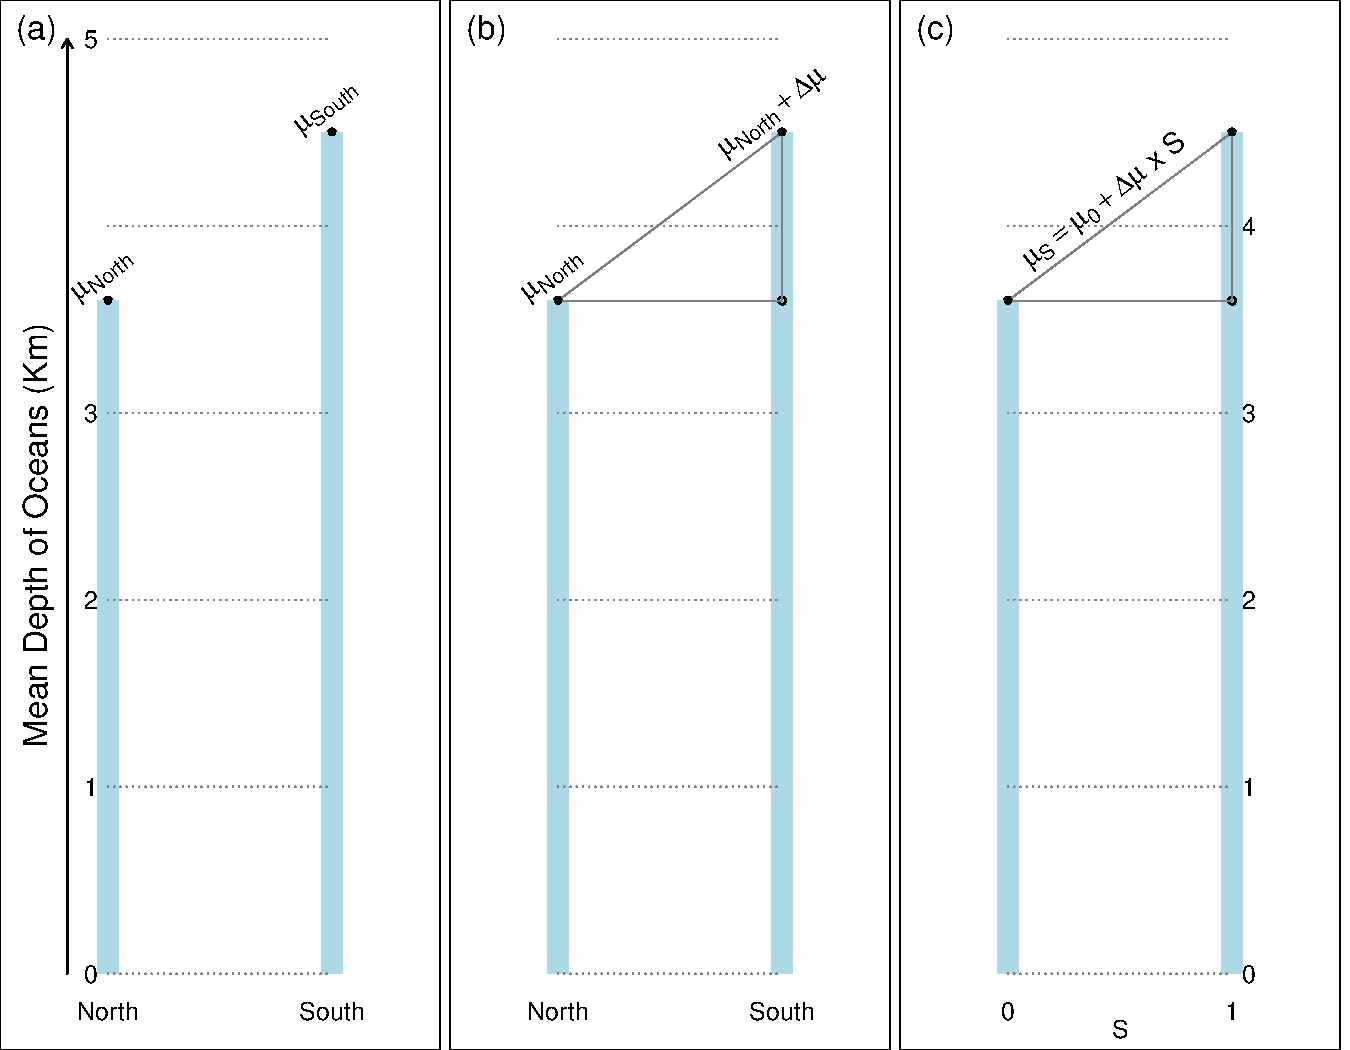
\includegraphics[width=\maxwidth]{figure/unnamed-chunk-17-1} 

}


\end{knitrout}
\end{frame}




\begin{frame}{Relative differences (ratios) - in numbers}
\begin{itemize}
	\item A ratio can be more helpful than a difference, especially if you are don't have a sense of how large the parameter value is even in the reference category. As an example, on average, how many more red blood cells do men have than women? or how much faster  are gamers' reaction times compared with nongamers?
\pause 
\item Recall our hypothetical mean ocean depths, 3.6 Km  in the 
oceans in the Northern hemisphere (reference category) and 4.5Km in the oceans of the Southern hemisphere (index category). Thus, the S:N (South divided by North) ratio is 4.5/3.6 or 1.25.
\pause 
\item Panel (a) leaves it to the reader to calculate the ratio of the parameter values. In panel (b)  the ratio (the quantity of interest) is isolated:  again, the original 2 parameters are converted to 2 new, more relevant ones. 
\pause 
\item Again, panel (c) shows a single master-equation that applies to both hemispheres by togging off/on the ratio of 4.5/3.6.
\end{itemize}
\end{frame}


\begin{frame}[fragile,plain]
\begin{knitrout}\tiny
\definecolor{shadecolor}{rgb}{0.969, 0.969, 0.969}\color{fgcolor}

{\centering 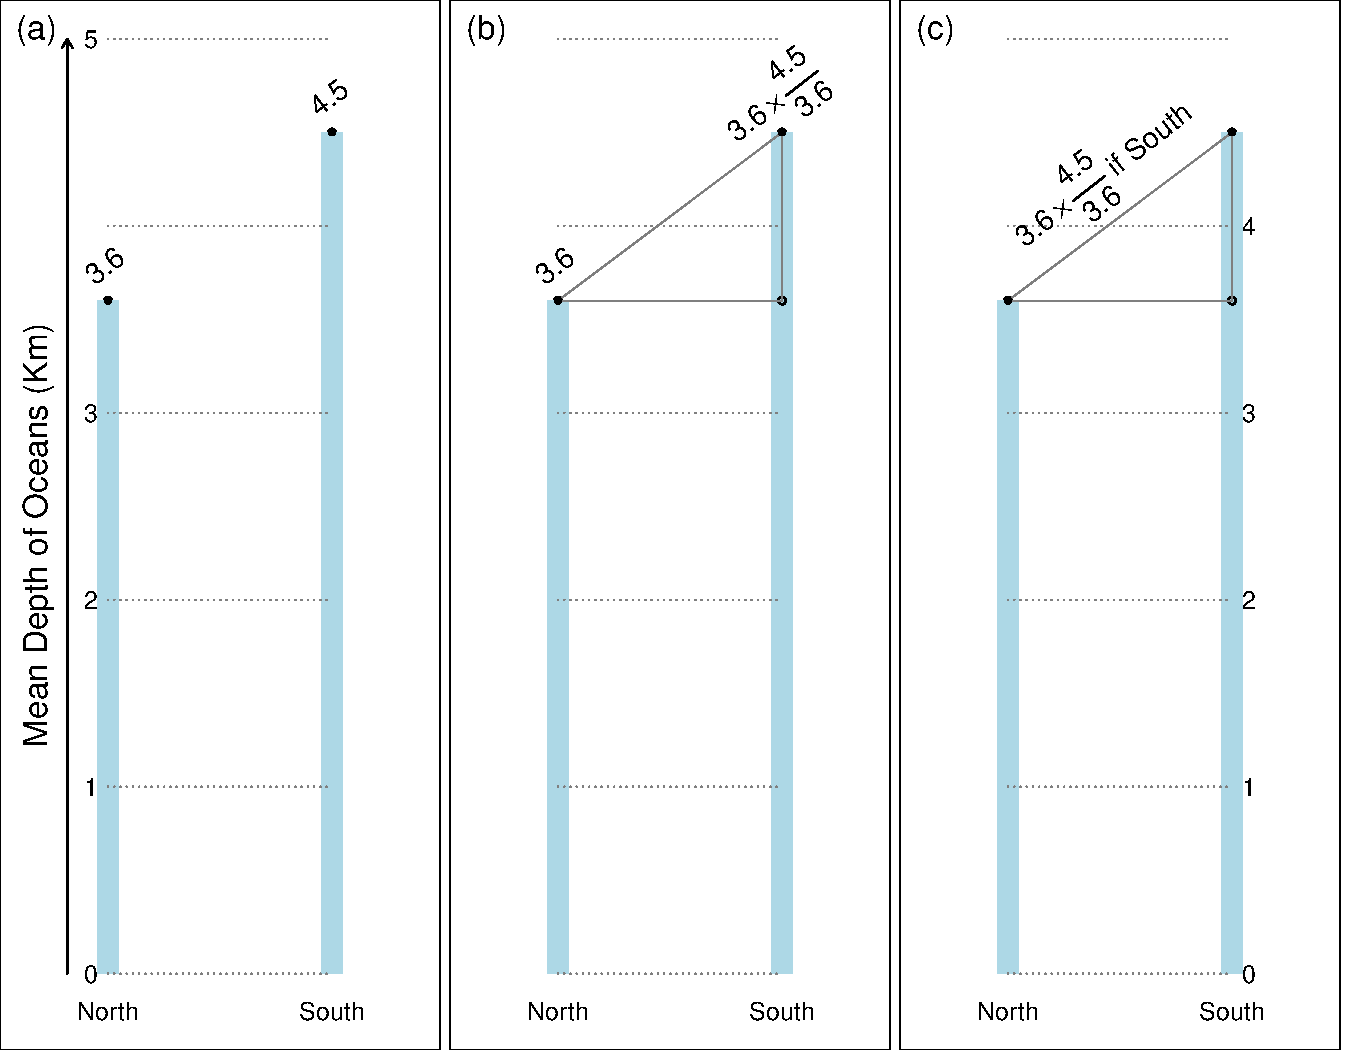
\includegraphics[width=\maxwidth]{figure/unnamed-chunk-18-1} 

}


\end{knitrout}
\end{frame}





\begin{frame}{Relative differences (ratios) - expressed in symbols}
	\begin{itemize}
		\item To rewrite these numbers in a symbolic equation suitable for a computer, we  again convert the logical 'if South' to a numerical Southern-hemisphere-indicator, using the binary variate $S$ (short for Southern) that takes the value 0 if the Northern hemisphere, and  1 if the Southern hemisphere.
		\pause 
	\item 	But go back to  some long-forgotten mathematics from high school to be able to tell the computer to toggle the ratio off and on. Recall \textbf{powers} of numbers, where, for example, 
		'$y$ to the power 2', or $y^2$ is the square of $y$. The two powers we exploit are 0 and 1.
		'$y$ to the power 1', or $y^1$ is just $y$ and '$y$ to the power 0', or $y^0$ is 1.
		\pause 		
\item 		We take advantage of these to write
		$$\mu_S = \mu \ | \ S  \ = \mu_0 \ \times \  \Big\{ \frac{\mu_{South}}{\mu_{North}}\Big\}^S = \mu_0 \ \times Ratio \ ^ S.$$ 
		
	\item 	You can check that it works for each hemisphere by setting $S=0$ and $S=1$ in turn. Thus, $$\log(y^S) = S \times \log(y)$$  
		
	\end{itemize}
\end{frame}


\begin{frame}[fragile,plain]
\begin{knitrout}\tiny
\definecolor{shadecolor}{rgb}{0.969, 0.969, 0.969}\color{fgcolor}

{\centering 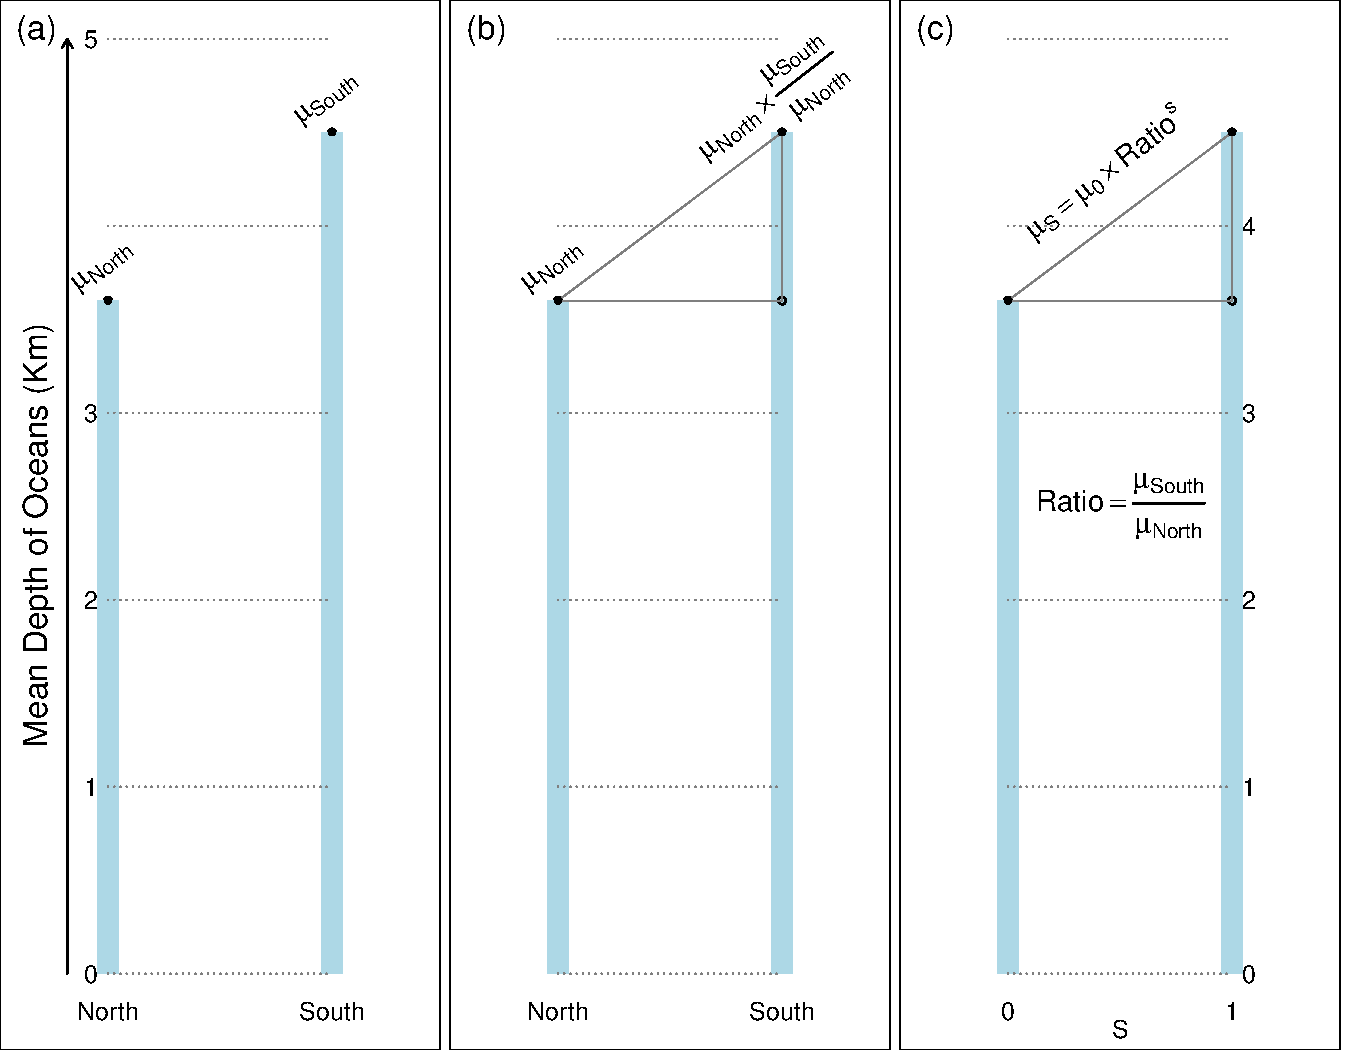
\includegraphics[width=\maxwidth]{figure/unnamed-chunk-19-1} 

}


\end{knitrout}
\end{frame}



\begin{frame}
\begin{itemize}
	\item Although this is a compact and direct way to express the
	parameter relation, it is not well suited for fitting these equations to data. 
	
\item 	However, in those same  high school mathematics courses, you also learned about \textbf{logarithms}. For example, that 
	$$\log(A \times B) = \log(A) + \log(B); \ \  \log(y^x) = x \times \log(y).$$
	\pause 
	\item Thus, we can rewrite the equation in panel (c) as
	
	$$\log(\mu_S) = \log(\mu \ | \ S)  \ = \underbrace{\log(\mu_0)} \ +  \underbrace{\log(Ratio)} \times \ S.$$
	
	\item This has the same 'linear in the two parameters' form as the one for the parameter difference: the parameters are
	$\underbrace{\log(\mu_0)}$ and $\underbrace{\log(Ratio)}$ and they are made into the following 'linear compound' or 'linear predictor' (see Remarks below) :
	$$\log(\mu_S) = \log(\mu \ | \ S)  \ = \underbrace{\log(\mu_0)} \times \ 1 \ + \underbrace{\log(Ratio)} \times \ S.$$
	\pause 
\item 	The course is concerned with using 'regression' software to  'fit'/'estimate' these 2 parameters from $n$ depth measurements indexed by $S$.
	
\end{itemize}
\end{frame}


\begin{frame}{Parameter Functions}
\begin{itemize}
	\item A very simple example of a function that describes how  parameter values vary over quantitative levels of a determinant is the straight line shown in the upper right panel of the next figure. Here the determinant has the generic name X, and the equation is of the $A + B \times X$ or $B_0 + B_1 \times X$ or $\beta_0 + \beta_1 \times X$ straight line form. 
	
	\item Miettinen used the convention that the upper case letters $A$ and $B$ are used to denote the (true but unknown) coefficient values, whereas the lower case leters $a$ and $b$ are used to denote their empirical counterparts, sometimes called estimated coefficients or fitted coefficients.  This sensible and simple convention also avoids the need, if one uses Greek letters for the theoretical coefficient values, to put 'hats' on them when we refer to their empirical counterparts, or 'estimate/fit' them. Fortunately, journals don't usually allow investigators to use 'beta-hats'; but this means that the investigators have to be more careful with their words and terms.
	

\end{itemize}
\end{frame}


\begin{frame}{Parameter Functions}
	\begin{itemize}
		
		\item As we go left to right in the following grid, the models become more complex. The simplest  is the one of the left, in column 1, the one  JH refers to as 'the mother of all regression models.'  It refers to a \textit{single} or \textit{overall} situation/population/domain, so $X \equiv 1$, it takes on the value 1 in/for every instance/member. 
		
		
		\item So the parameter equation is $\mu_X = \mu \ | \ X \ = \mu \times 1.$ In column 2, there are 2 subdomains, indexed by the 2 values of  the determinant (here generically called 'X'), namely $X = 0$ and $X = 1$. In the 3rd column, the number of of parameters is left unspecified, since the numbers of coefficients to specify a line/curve might vary from as few as 1 (if we were describing how the volume of a cube dependeds or, was is function of, its radius) to 2 (for a straight line that did not go through the origin, or for a symmetric S curve) to \textit{more than 2} (e.g., for a non-symmetric S curve, or a quadratic shape).
	\end{itemize}
\end{frame}


\begin{frame}[fragile,plain]
\begin{knitrout}\tiny
\definecolor{shadecolor}{rgb}{0.969, 0.969, 0.969}\color{fgcolor}

{\centering 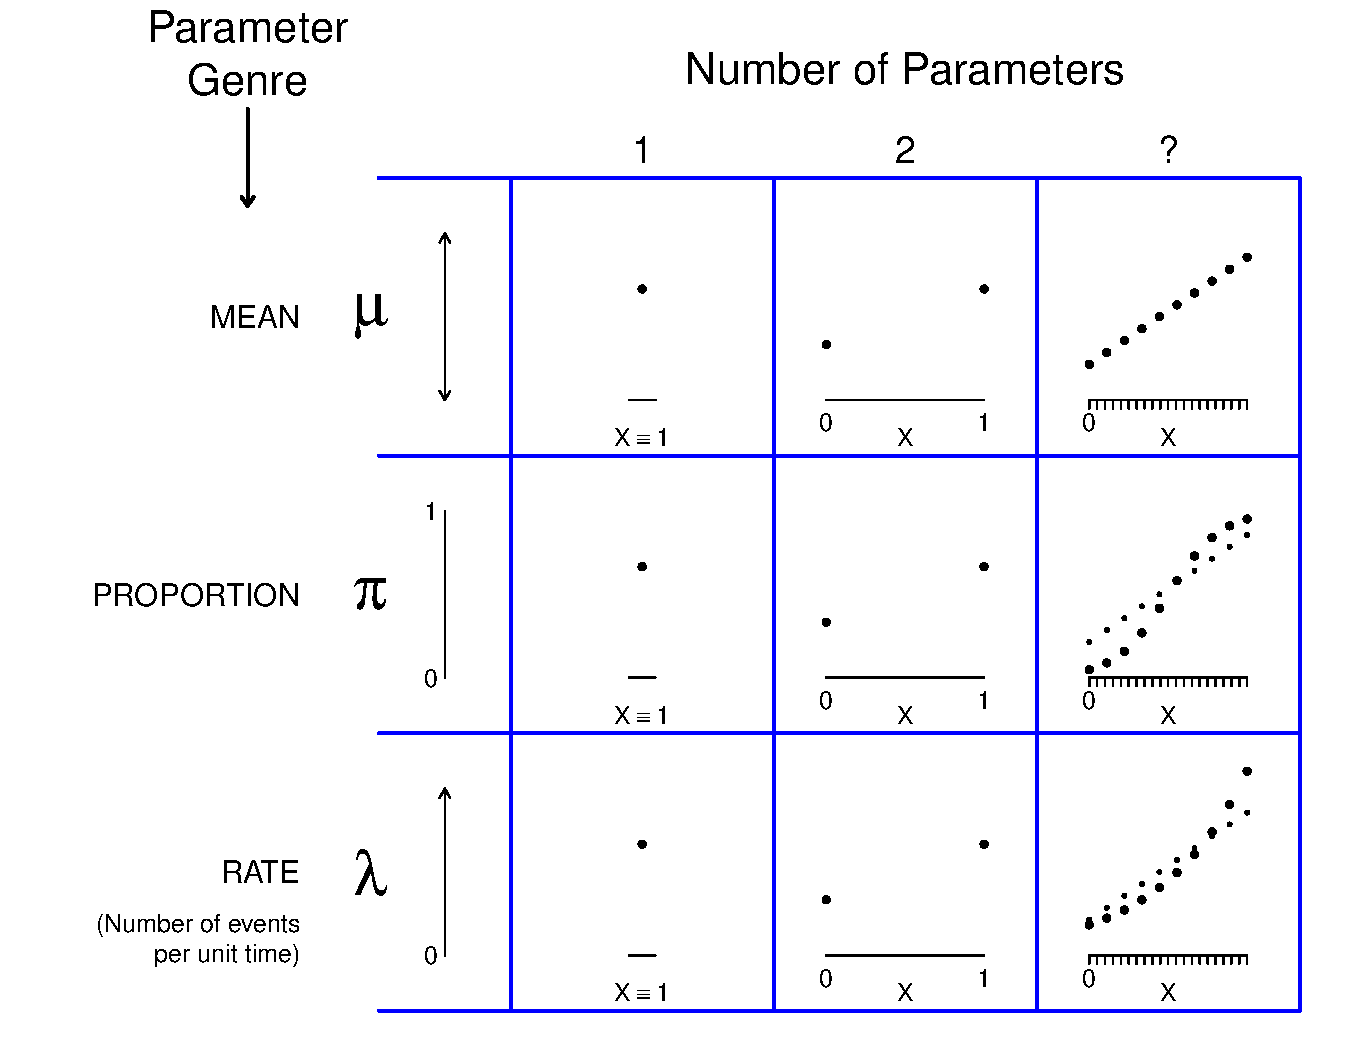
\includegraphics[width=\maxwidth]{figure/unnamed-chunk-20-1} 

}


\end{knitrout}
\end{frame}


\end{document}


